%%%%%%%%%%%%%%%%%%%%%%%%%%%%%%%%%%%%%%%%%%%%%%%%%%%%%%%%%%%%%%%%%%%%%%%%%%%%%%%%
%2345678901234567890123456789012345678901234567890123456789012345678901234567890
%        1         2         3         4         5         6         7         8


\documentclass[letterpaper, 10 pt, conference]{ieeeconf}  % Comment this line out
                                                          % if you need a4paper
%\documentclass[a4paper, 10pt, conference]{ieeeconf}      % Use this line for a4
                                                          % paper

\IEEEoverridecommandlockouts                              % This command is only
                                                          % needed if you want to
                                                          % use the \thanks command
\overrideIEEEmargins
% See the \addtolength command later in the file to balance the column lengths
% on the last page of the document

\usepackage{graphicx}
\usepackage{float}
\usepackage{graphics}
\usepackage[utf8]{inputenc}
%\usepackage[spanish, activeaccute]{babel} %permite escribir con ortografía en español, acentos, ñ, etc
\usepackage[spanish,es-noshorthands]{babel}
\usepackage{mathtools} %matematica
\usepackage{amsmath} %matematica
\usepackage{circuitikz} %pa dibujar circuitoz
\usepackage{siunitx} %simbologia, ohm etc
\usepackage{amssymb}
\usepackage{hyperref}


% Para los acentos
%\usepackage[spanish]{babel}
% The following packages can be found on http:\\www.ctan.org
%\usepackage{graphics} % for pdf, bitmapped graphics files
%\usepackage{epsfig} % for postscript graphics files
%\usepackage{mathptmx} % assumes new font selection scheme installed
%\usepackage{times} % assumes new font selection scheme installed
%\usepackage{amsmath} % assumes amsmath package installed
%\usepackage{amssymb}  % assumes amsmath package installed

\title{\LARGE \bf
Laboratorio 4 - Circuitos Electrónicos I - Ing. Electrónica
}

%\author{ \parbox{3 in}{\centering Huibert Kwakernaak*
%         \thanks{*Use the $\backslash$thanks command to put information here}\\
%         Faculty of Electrical Engineering, Mathematics and Computer Science\\
%         University of Twente\\
%         7500 AE Enschede, The Netherlands\\
%         {\tt\small h.kwakernaak@autsubmit.com}}
%         \hspace*{ 0.5 in}
%         \parbox{3 in}{ \centering Pradeep Misra**
%         \thanks{**The footnote marks may be inserted manually}\\
%        Department of Electrical Engineering \\
%         Wright State University\\
%         Dayton, OH 45435, USA\\
%         {\tt\small pmisra@cs.wright.edu}}
%}

\author{Ignacio Nahuel Chantiri 69869/1 \\  %\vspace{1cm}
{\it Universidad Nacional De La Plata, Argentina,}
{\it Julio 2024.}}                              % <-this % stops a space

\begin{document}


\maketitle
\thispagestyle{empty}
\pagestyle{empty}


%%%%%%%%%%%%%%%%%%%%%%%%%%%%%%%%%%%%%%%%%%%%%%%%%%%%%%%%%%%%%%%%%%%%%%%%%%%%%%%%
\begin{abstract}

El análisis de laboratorio presentado describe el estudio de un amplificador en configuración Cascode. Se propuso como objetivo verificar el comportamiento a frecuencias medias y altas y compararlo con una etapa simple de Emisor Común.
\end{abstract}


%%%%%%%%%%%%%%%%%%%%%%%%%%%%%%%%%%%%%%%%%%%%%%%%%%%%%%%%%%%%%%%%%%%%%%%%%%%%%%%%
\section{Introducci\'on}

El informe posee el siguiente formato:\\
Primeramente, incluye un \textit{Marco Teórico} que abarca las explicaciones y describe el comportamiento esperado.\\ A continuación, se presenta el \textit{Desarrollo experimental}, con la descripción del set-up y conexiones de la placa, junto con los resultados y mediciones correspondientes, seguido finalmente de una conclusión y comparación con las cuentas analíticas para cada uno de los pasos realizados.


\section{Marco teórico}

La placa utilizada es la diagramada en la Figura \autoref{fig:diagramaplaca}.

\begin{figure}[H]
  \centering
  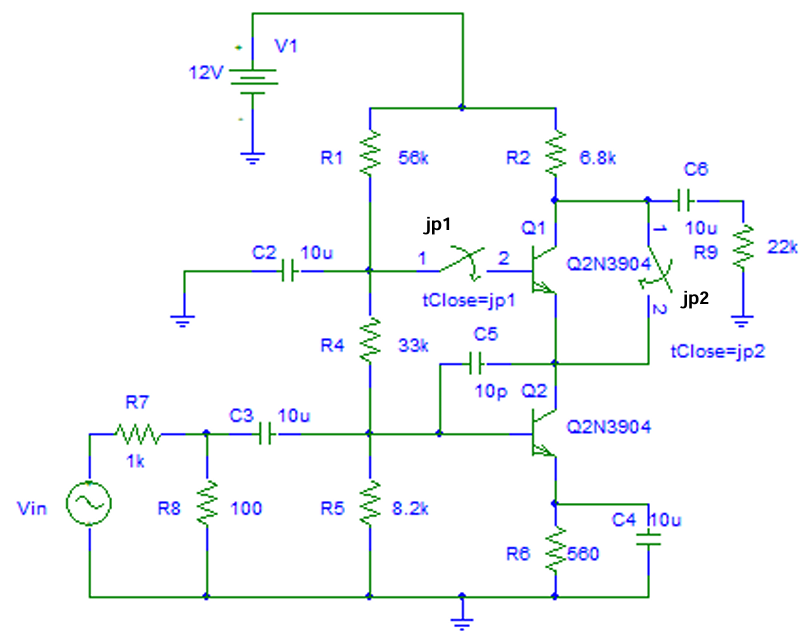
\includegraphics[width=0.47\textwidth]{imagenes/placa.png}
  \caption{Diagrama circuital de la placa utilizada.}
  \label{fig:diagramaplaca}
\end{figure}

Se compone de una configuración Cascode con dos jumpers (jp1 y jp2) que deja en uso el Cascode, o permite saltearse la etapa de Base Común, dejando en operación solamente la etapa de Emisor Común.
Esto permitirá analizar la Ganancia de Tensión y el Ancho de Banda para ambos casos, solamente abriendo o cerrando los jumpers.

\subsection{\textbf{Aproximación del polo dominante y Método de las Constantes de Tiempo.}}

Obtener la frecuencia de corte por medio de la transferencia de un amplificador puede ser una tarea engorrosa, por lo que para simplificar el análisis, se considera que la respuesta en frecuencia del circuito está dado solamente por el comportamiento del polo más bajo.
Para ello se asume que la frecuencia del polo más bajo es mucho menor que la del polo que le sigue, de modo que mientras más separados estén los polos, mejor es la aproximación.\\
Una tranferencia genérica de tres polos reales y ningún cero finito tendrá la siguiente forma:

\begin{equation}
A = \frac{A_0}{(1+s/p_1)(1+s/p_2)(1+s/p_3)} 
\end{equation}

\begin{equation}
A = \frac{A_0}{1 + a_1s + a_2s^2 + a_3s^3}
\end{equation}

Donde $A_0$ es la ganancia de continua.\\
Se tiene entonces:

\begin{equation}
\left\{
\begin{aligned}
a_1 &= \frac{1}{p_1} + \frac{1}{p_2}  + \frac{1}{p_3} \\ 
a_2 &= \frac{1}{p_1.p_2} + \frac{1}{p_1.p_3} + \frac{1}{p_2.p_3}\\
a_3 &= \frac{1}{p_1.p_2.p_3}\\
\end{aligned}
\right.
\end{equation}

Ahora, considerando $p_1<<p_2<<p_3$ se llega a la expresión final de los polos en función de los coeficientess $a_i$:

\begin{equation}
\left\{
\begin{aligned}
p_1 &\approx \frac{1}{a_1}\\ 
p_2 &\approx \frac{a_1}{a_2} \\
p_3 &\approx \frac{a_2}{a_3}\\
\end{aligned}
\right.
\label{eq:aprox_polos}
\end{equation}

Haciendo uso de estás últimas expresiones, nos interesa particularmente la ubicación del polo dominante $p_1$. Para hallarlo, necesitamos saber el valor de $a_1$.
Si se considera que el circuito visto desde los terminales de los capacitores existentes contiene sólo resistencias y fuentes dependientes, la transferencia para un circuito de tres polos se puede resescribir como:

\begin{equation}
a_1 = C_1R_{11}^0 + C_2R_{22}^0 + C_3R_{33}^0\\
\end{equation}

Donde $R_{11}^0$, $R_{22}^0$ y $R_{3}^0$ son las impedancias vistas desde los capacitores $C_1$, $C_2$ y $C_3$ a frecuencia cero.
Como expresión general para N capacitores, se expresa el coeficiente $a_1$ como:

\begin{equation}
a_1 = \sum_{i=1}^N C_iR_{ii}^0
\label{eq:formula_a1}
\end{equation}

En resumen, se puede expresar $a_1$ como la suma de las constantes de tiempo de cada capacitor individual cuando el resto de los capacitores están a circuito abierto. \\
Esta expresión es sumamente útil para aproximar la frecuencia de corte de un circuito multietapa como el que se analiza en este laboratorio, simplemente calculando la inversa de $a_1$ según lo visto en la ecuación \ref{eq:formula_a1}.

\subsection{\textbf{Tiempo de respuesta (tiempo de subida)}}

Se denomina \textit{Tiempo de subida} o \textit{Tiempo de respuesta} al tiempo que tarda en reaccionar la señal de salida $V_o$ ante un escalón en la entrada. Generalmente, se mide el intervalo de tiempo que tarda en tomar entre el 10\% y el 90\% de su valor final; por lo que es un indicador de cuán rápido puede responder el amplificador a una discontinuidad en la tensión de entrada.
Para un circuito de un solo polo, el tiempo de respuesta $t_r$ se relaciona con la frecuencia de corte según:

\begin{equation}
    t_r = \frac{0.35}{f_H}\\
\end{equation}

Esta fórmula es válida como aproximación para un circuito con más de un polo, como es el caso.

\subsection{\textbf{Configuración Cascode.}}

La configuración Cascode tiene como objetivo el aumento de la impedancia de salida, y reducir el efecto de la capacidad de Miller, responsable de la limitación del Ancho de Banda del amplificador.\\
Para lograrlo, se colocan en cascada un par de transistores idénticos (idealmente), uno en Emisor Común y el otro en Base Común, en ese orden.

\begin{figure}[H]
  \centering
  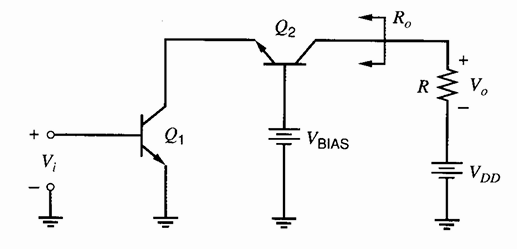
\includegraphics[width=0.47\textwidth]{imagenes/cascode basico.png}
  \caption{Configuración cascode.}
  \label{fig:cascode}
\end{figure}

A continuación, se procede a analizar la placa diagramada en la Figura \ref{fig:diagramaplaca} en sus dos configuraciones posibles.

\subsection{\textbf{Análisis de la Placa en Emisor Común. (jp1 abierto, jp2 cerrado)}}

El circuito de la Figura es un equiivalente a dejar el jp1 abierto y el jp2 cerrado.

\begin{figure}[H]
  \centering
  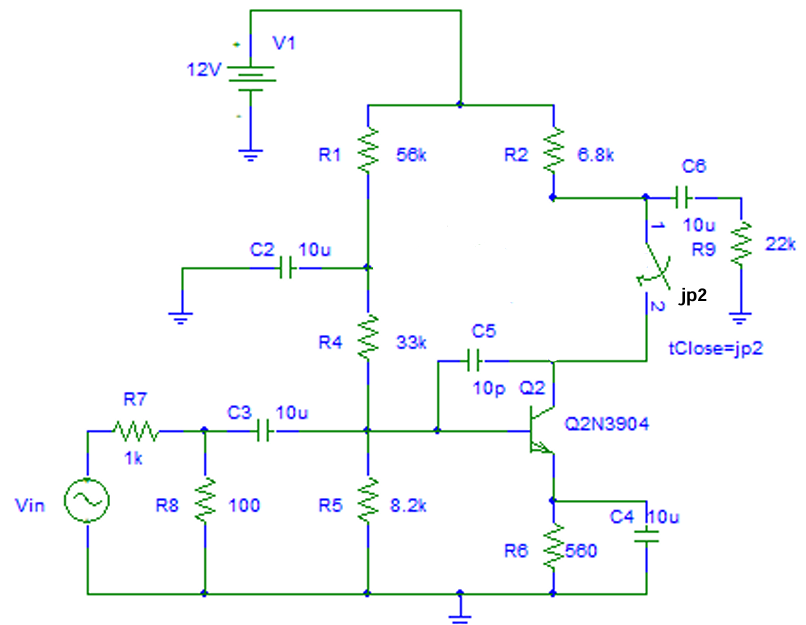
\includegraphics[width=0.47\textwidth]{imagenes/diagrama polarizacion ec.png}
  \caption{Equivalente al circuito de la placa para polarización, con jp1 abierto y jp2 cerrado.}
  \label{fig:pola_ec}
\end{figure}

\subsubsection{Polarización del EC}
Para los datos de la placa:\\
$V_{cc} = 12V$, $\beta = 200$, $f_t = 270MHz$, $C_{\mu} = 4pF$\\
Se obtuvieron los siguientes valores de polarización:\\

\begin{itemize}
    \item $V_{e} = V_b - 0.7V = 12V \cdot \frac{8.2k\Omega}{8.2k\Omega + 33k\Omega + 58k\Omega} -0.7V \approx 0.29V$\\
    \item $I_{cq} = \frac{V_e}{R_e} = \frac{0.29V}{560\Omega} \approx 521 \mu A$\\
    \item $V_{ce} = V_{cc} - I_{cq}R_c - V_e = 12V - (6.8k\Omega)(521 \mu A) - 0.29V \approx 8.16V$\\
    \item $g_m = \frac{I_{cq}}{V_T} = \frac{521\mu A}{26mV} = 20.03m$\\
    \item $r_{\pi} = \frac{\beta}{g_m} = \frac{200}{20.03m} = 10k\Omega$\\
\end{itemize}




\subsubsection{Respuesta del EC a frecuencias medias}
Para el análisis a frecuencias medias, se ignora el comportamiento capacitivo del transistor. El circuito final de frecuencias medias queda representado por el diagrama de la Figura \ref{fig:ECfreq_medias}

\begin{figure}[H]
  \centering
  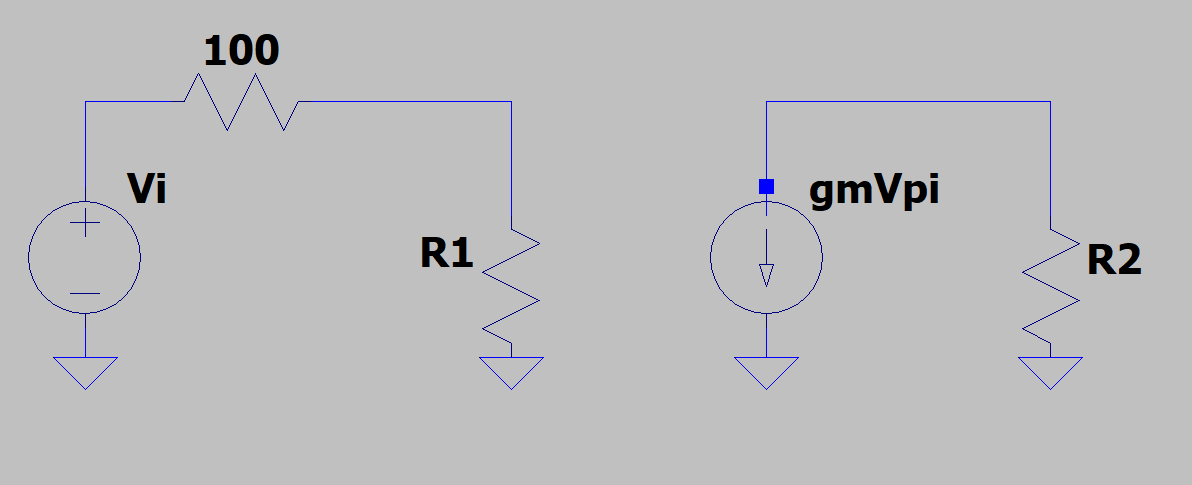
\includegraphics[width=0.47\textwidth]{imagenes/freq medias EC.png}
  \caption{Equivalente al circuito de la placa para frecuencias medias, con jp1 abierto y jp2 cerrado.}
  \label{fig:ECfreq_medias}
\end{figure}

Con el modelo de pequeña señal de este circuito, se plantea el siguiente sistema de ecuaciones:\\

\begin{equation}
\left\{
\begin{aligned}
V_o &= -gmV_{\pi }R_2\Omega\\ 
V_{\pi} &= \frac{V_iR_1}{R_1 + 1k\Omega}\\
\end{aligned}
\right.
\label{aprox_polos}
\end{equation}

Siendo:

\begin{equation}
    R_1 = (r_{\pi} // 33k // 8,2k // 100) \Omega \approx 97,5\Omega\\
\end{equation}

y

\begin{equation} 
    R_2 = (22k // 8,8k) \Omega \approx 5,2k\Omega.      
\end{equation}

La ganancia de Tensión $A_v$ para el EC queda expresada como:\\
\begin{equation}
A_v = \frac{V_o}{V_i} = \frac{-gmR_1R_2\Omega}{R_1 + 1k\Omega}\\
\end{equation}

Resolviendo:

\begin{equation}
A_v = -9.2554\\
\end{equation}

\subsubsection{Respuesta del EC a frecuencias altas}

Para el análisis a frecuencias altas se considera también el comportamiento capacitivo del transistor. El circuito final de frecuencias altas queda representado por el diagrama de la Figura \ref{fig:ECfreq_altas}.

\begin{figure}[H]
  \centering
  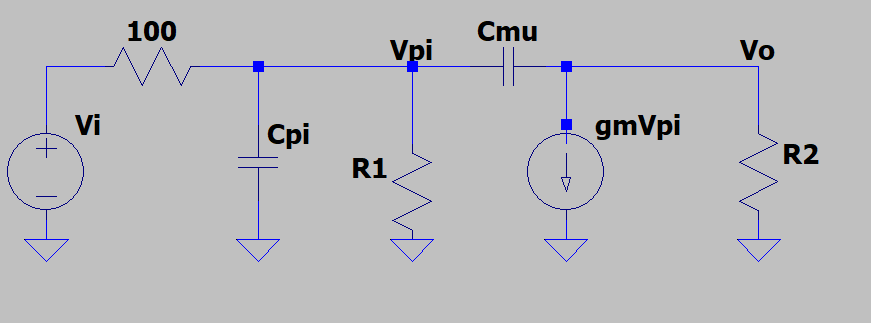
\includegraphics[width=0.47\textwidth]{imagenes/freq altas EC.png}
  \caption{Equivalente al circuito de la placa para frecuencias altas, con jp1 abierto y jp2 cerrado.}
  \label{fig:ECfreq_altas}
\end{figure}

Se procede al análisis por método de las constantes de tiempo.

La resistencia $R_{\pi}^0$ vista desde el capacitor $C_\pi$ con el capacitor $C_\mu$ a circuito abierto es:

\begin{equation}
    R_{\pi}^0 = 1k\Omega // R_1 = 1k\Omega // 97,5\Omega \approx 88,86\Omega
\end{equation}

La resistencia $R_{\mu}^0$ vista desde el capacitor $C_\pi$ con el capacitor $C_\pi$ a circuito abierto es:

\begin{equation}
    R_{\mu}^0 = R_{\pi}^0(1 + gmR_2) + R_2 \approx 14,53 k\Omega
\end{equation}

Siendo $R_2 = 6,8k\Omega // 22k\Omega \approx 5,2k\Omega$ \\

El coeficiente $a_1$ será:

\begin{equation}
    a_1 = C_\pi R_{\pi}^0 + C_\mu  R_{\mu}^0 
\end{equation}

Para $ C_\pi = 585,46pF$ y $C_\mu = 4pF$:

\begin{equation}
    a_1 \approx 0,1118\mu s
\end{equation}

La frecuencia de corte será $\frac{1}{a_1}$:

\begin{equation}
    w_H = \frac{1}{0,1101\mu s} \approx 9,07M \frac{rad}{s}\\
\end{equation}
\begin{equation}
    f_H = \frac{w_H}{2\pi} \approx 1,444MHz
\end{equation}

\subsubsection{Tiempo de respuesta del EC}
Para el Emisor Común, el tiempo de respuesta con la frecuencia de corte calculada será:

\begin{equation}
    t_r = \frac{0,35}{f_H} = \frac{0,35}{1,444MHz} \approx 242,3ns
\end{equation}

\subsection{\textbf{Análisis de la Placa en Cascode. (jp1 cerrado, jp2 abierto)}}

\subsubsection{Polarización del Cascode}

La corriente de polarización $I_{cq}$ está dada por la $V_{be}$ y la $R_e$ del emisor común, por lo que los valores de polarización son similares.

\subsubsection{Respuesta del Cascode a frecuencias medias}

Del modelo de pequeña señal del Cascode (Figura \ref{fig:cascode_freq_medias}) se puede derivar el siguiente sistema de ecuaciones:

\begin{equation}
\left\{
\begin{aligned}
V_o &= -gmV_{\pi 2}R_2\\ 
V_{\pi2} &= \frac{gmV_{\pi1}}{gm+r_{\pi2}^{-1}} \\
V_{\pi1} &= \frac{V_iR_1}{(R_1 + 1k\Omega)}\\
\end{aligned}
\right.
\label{aprox_polos}
\end{equation}

Siendo:

\begin{equation}
    R_1 = (r_{\pi} // 33k // 8,2k // 100) \Omega \approx 97,5\Omega
\end{equation}

y

\begin{equation} 
    R_2 = (22k // 8,8k) \Omega \approx 5,2k\Omega.      
\end{equation}

\begin{figure}[H]
  \centering
  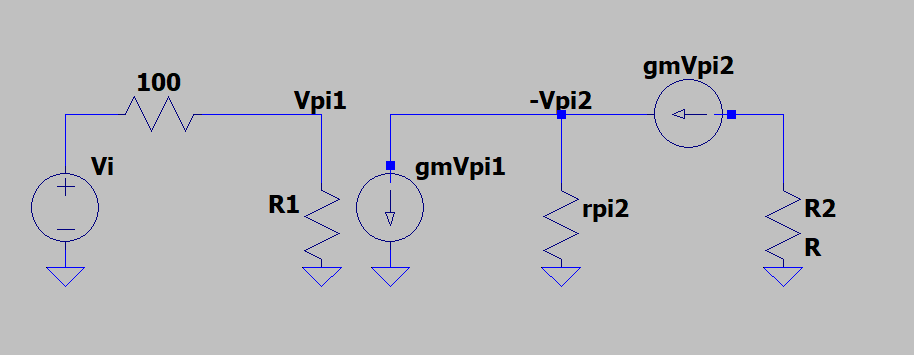
\includegraphics[width=0.47\textwidth]{imagenes/freq medias cascode.png}
  \caption{Equivalente al circuito de la placa para frecuencias altas, con jp1 abierto y jp2 cerrado.}
  \label{fig:cascode_freq_medias}
\end{figure}

La ganancia de Tensión $A_v$ para el Cascode queda expresada como:\\
\begin{equation}
A_v = \frac{V_o}{V_i} = \frac{-gm^2R_1R_2}{(R_1 + 1k\Omega)(gm+r_{\pi2}^{-1})} \approx -9,2\\
\end{equation}

\subsubsection{Respuesta del Cascode a frecuencias altas}

Para el análisis a frecuencias altas se considera también el comportamiento capacitivo de los transistores. El circuito final de frecuencias altas queda representado por el diagrama de la Figura \ref{fig:cascode_freq_altas}.

\begin{figure}[H]
  \centering
  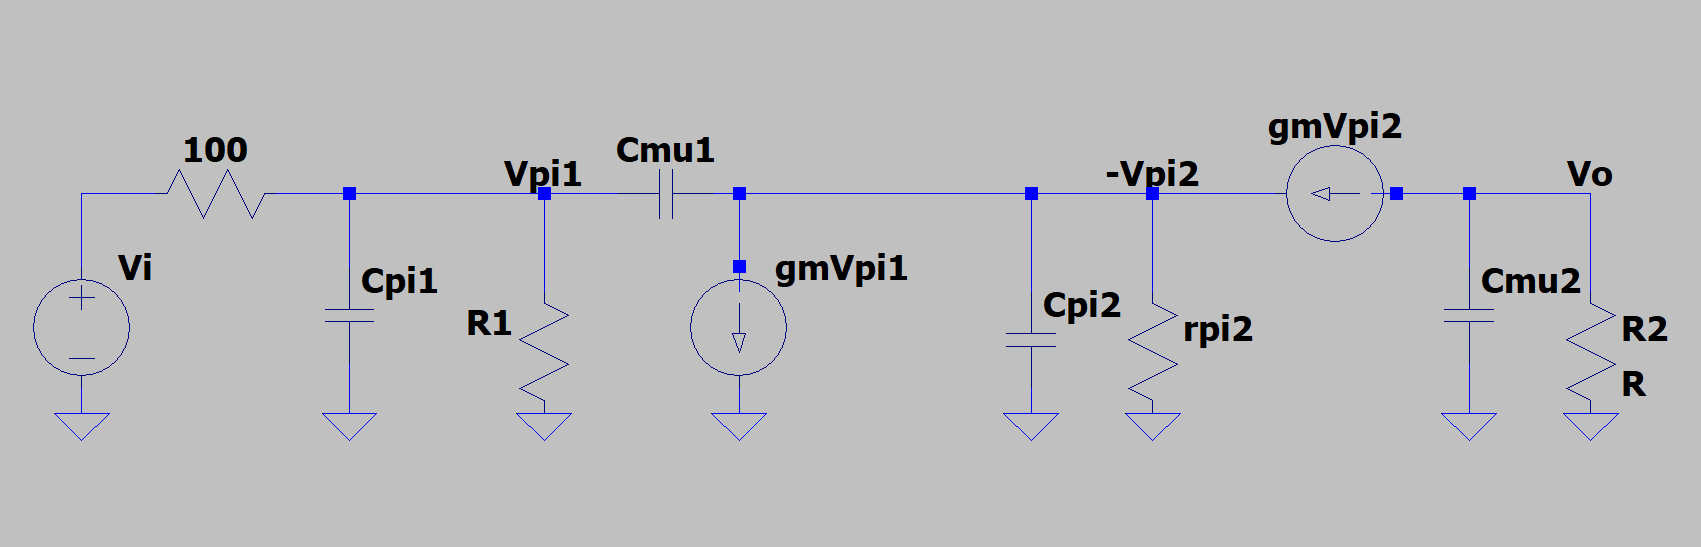
\includegraphics[width=0.47\textwidth]{imagenes/freq acltas cascode.png}
  \caption{Equivalente al circuito de la placa para frecuencias altas, con jp1 abierto y jp2 cerrado.}
  \label{fig:cascode_freq_altas}
\end{figure}

Se procede al análisis por método de las constantes de tiempo.

La resistencia $R_{\pi1}^0$ vista desde el capacitor $C_{\pi1}$ con el resto de los capacitores a circuito abierto es:

\begin{equation}
    R_{\pi1}^0 = 1k\Omega \parallel R_1 = 1k\Omega \parallel 97,5\Omega \approx 88,86\Omega
\end{equation}

La resistencia $R_{\pi2}^0$ vista desde el capacitor $C_{\pi2}$ con el resto de los capacitores a circuito abierto es:

\begin{equation}
    R_{\pi2}^0 = r_{\pi2} \parallel (Z + R_2) \approx 49,62\Omega
\end{equation}

La resistencia $R_{\mu1}^0$ vista desde el capacitor $C_{\mu1}$ con el resto de los capacitores a circuito abierto es:

\begin{equation}
    R_{\mu1}^0 = R_{\pi2}^0(1 + gmR_{\pi1}^0) + R_{\pi1}^0 \approx 226,9\Omega
\end{equation}

La resistencia $R_{\mu2}^0$ vista desde el capacitor $C_{\mu2}$ con el resto de los capacitores a circuito abierto es:

\begin{equation}
    R_{\mu2}^0 = (Z + r_{pi2})\parallel R_2 \approx 2.5 k\Omega
\end{equation}

Siendo:

\begin{equation}
\begin{aligned}
R_2 &= 6.8\,\text{k}\Omega \parallel 22\,\text{k}\Omega \approx 5.2\,\text{k}\Omega \\
R_1 &= (r_{\pi} \parallel 33\,\text{k}\Omega \parallel 8.2\,\text{k}\Omega \parallel 100\,\Omega) \approx 97,5\,\Omega \\
Z &= gm^{-1} - R2 
\end{aligned}
\end{equation}

Para el Cascode, el coeficiente $a_1$ será:

\begin{equation}
    a_1 = C_{\pi1} R_{\pi1}^0 + C_{\mu1}  R_{\mu1}^0 +  C_{\pi2} R_{\pi1}^0 + C_{\mu1}  R_{\mu1}^0 \\
\end{equation}

Para $ C_\pi = 585,46pF$ y $C_\mu = 4pF$:

\begin{equation}
    a_1 \approx 919,3\mu s
\end{equation}

La frecuencia de corte será $\frac{1}{a_1}$:

\begin{equation}
    w_H = \frac{1}{919,3\mu s} \approx 10,877M \frac{rad}{s}\\
\end{equation}
\begin{equation}
    f_H = \frac{w_H}{2\pi} \approx 1,731MHz
\end{equation}

\subsubsection{Tiempo de respuesta del Cascode}
Para el Cascode, el tiempo de respuesta con la frecuencia de corte calculada será:

\begin{equation}
    t_r = \frac{0,35}{f_H} = \frac{0,35}{3MHz} \approx 202,1ns
\end{equation}

\section{Desarrollo experimental}
Habiendo estudiado la placa de manera teórica previamente, se procedió a comprobar los resultados empíricamente.
Para todas las medidas de esta sección, la onda amarilla en el osciloscopio corresponde a la señal de entrada, mientras que la onda azul/celeste, corresponde a la de salida. Se polarizó la placa con una $V_{cc}$ de $12V$.
La señal de entrada es una sinusoide de $V_{max} = 100mV$.

\subsection{\textbf{Ganancia a Frecuencias Medias del Emisor Común }}

Se cerró el jp2 y se abrió el jp1, de manera que solo quede conectado el Emisor Común, y se midió la ganancia a un

\begin{figure}[H]
  \centering
  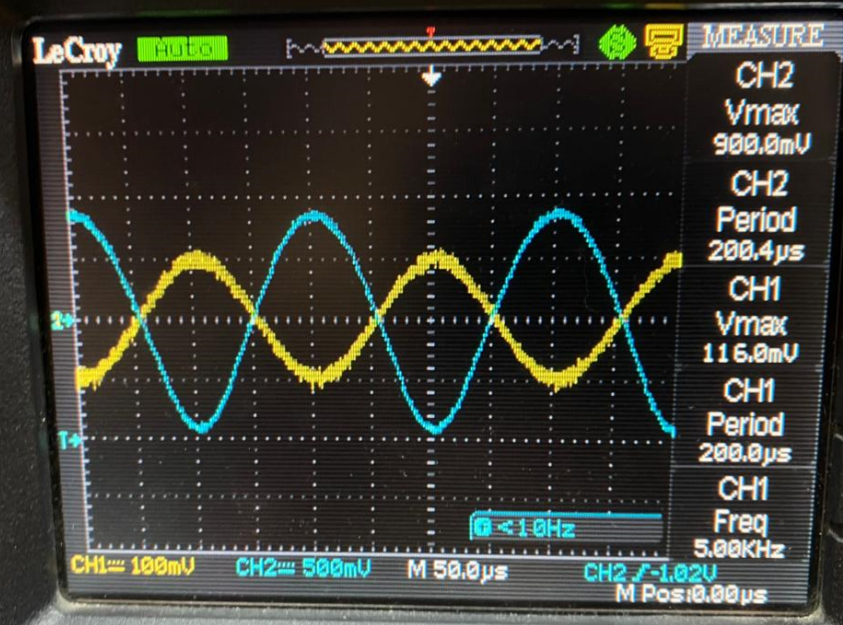
\includegraphics[width=0.47\textwidth]{imagenes/gananciaEC.png}
  \caption{Ganancia de la etapa del emisor común. Entrada en amarillo, salida en celeste.}
  \label{fig:ganancia_EC}
\end{figure}

La ganancia observada experimentalmente a frecuencias medias para el Emisor Común fue $A_v = \frac{900mV}{116mV} \approx 7.8 $

\subsection{\textbf{Frecuencia de corte $f_H$ del Emisor Común.}}

Para hallar la frecuencia de corte se buscó una atenuación de $3dB$ en la salida del amplificador. Esto es:

\begin{equation}
V_o = \frac{900mV}{\sqrt{2}} \approx 636mV \\
\end{equation}

\begin{figure}[H]
  \centering
  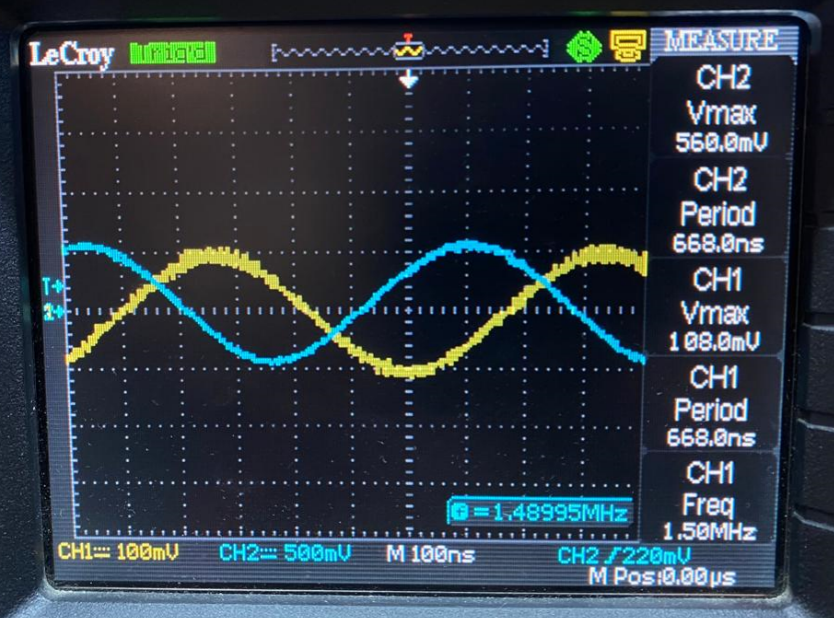
\includegraphics[width=0.47\textwidth]{imagenes/frecuencia_corte_EC.jpg}
  \caption{Se midió la frecuencia para una atenuación de 3dB (aproximadamente 636mV en la salida). Entrada en amarillo, salida en celeste.}
  \label{fig:freq_corte_EC}
\end{figure}

La frecuencia de corte medida para el Emisor Común fue $f_H = 1,49Mhz$

\subsection{\textbf{Respuesta temporal $t_r$ del Emisor Común.}}

El tiempo de respuesta $t_r$ se midió primeramente con la función de "Rise Time" del osciloscopio, a una frecuencia media, de $100kHz$. De todas maneras, se comprobó esa medición manualmente, posicionando los cursores entre el 10\% y el 90\% del valor final de $960mV$ (96mV y 864mV, respectivamente) y midiendo la diferencia de tiempo.\\


\begin{figure}[H]
  \centering
  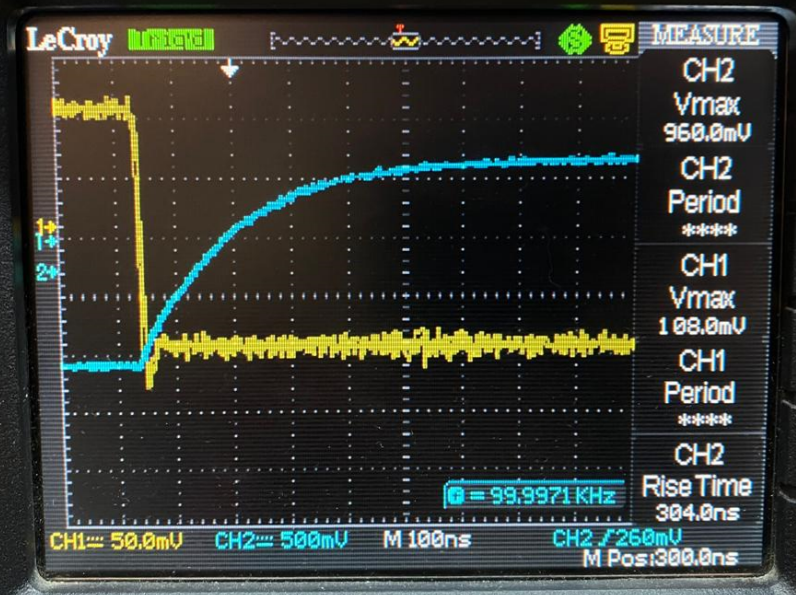
\includegraphics[width=0.47\textwidth]{imagenes/tiempo de respuesta EC.png}
  \caption{Se observa el tiempo de respuesta en la esquina inferior derecha, como "Rise Time"}
  \label{fig:tr_EC}
\end{figure}

El tiempo de respuesta medido para el Emisor Común fue $t_r = 304ns$.

\subsection{\textbf{Ganancia a Frecuencias Medias del Cascode.}}

Se abrió el jp2 y se cerró el jp1, de manera que quede el Emisor Común en cascada con el Base Común.

\begin{figure}[H]
  \centering
  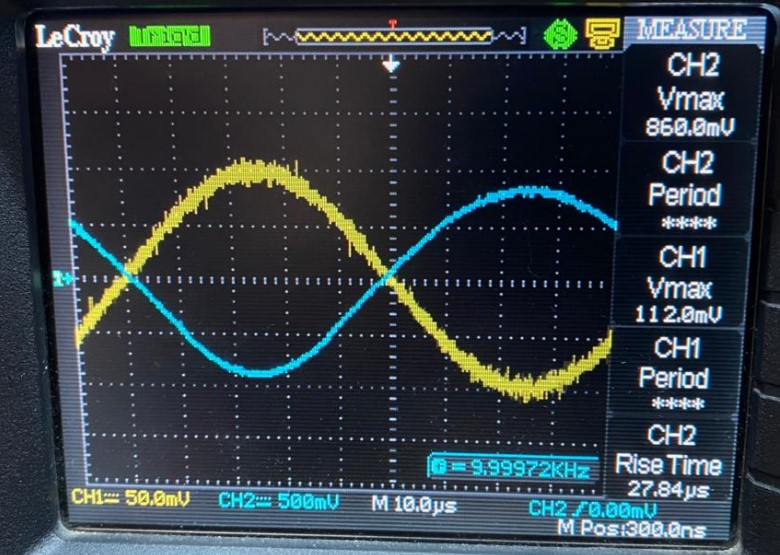
\includegraphics[width=0.47\textwidth]{imagenes/ganancia_cascode.jpg}
  \caption{Ganancia del Cascode. Entrada en amarillo, salida en celeste.}
  \label{fig:ganancia_EC}
\end{figure}

La ganancia observada experimentalmente a frecuencias medias para el Cascode fue $A_v = \frac{860mV}{112mV} \approx 7.7 $\\

\subsection{\textbf{Frecuencia de corte $f_H$ del Cascode.}}

Para hallar la frecuencia de corte se buscó una atenuación de $3dB$ en la salida del amplificador. Esto es:

\begin{equation}
V_o = \frac{860mV}{\sqrt{2}} \approx 608mV \\
\end{equation}

\begin{figure}[H]
  \centering
  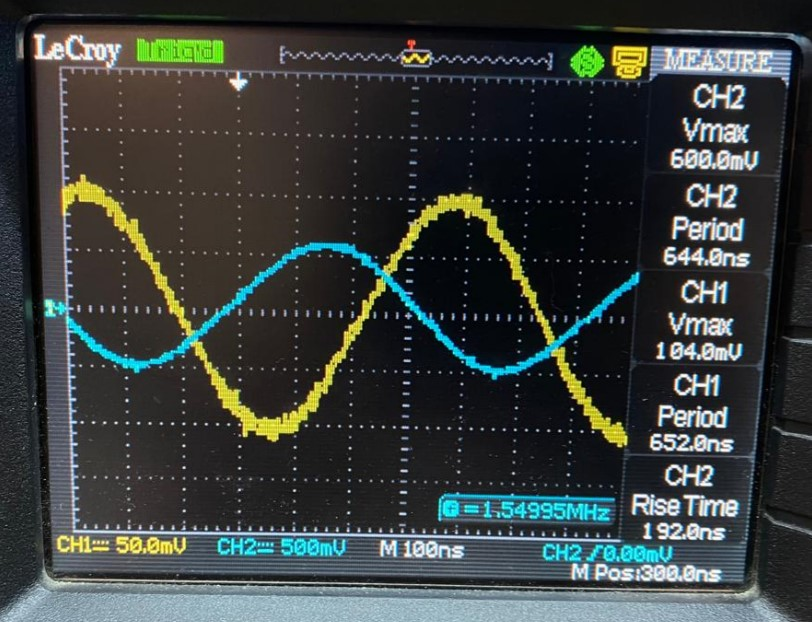
\includegraphics[width=0.47\textwidth]{imagenes/frecuencia_corte_CASCODE.jpg}
  \caption{Se midió la frecuencia para una atenuación de 3dB (aproximadamente 608mV en la salida). Entrada en amarillo, salida en celeste.}
  \label{fig:freq_corte_EC}
\end{figure}

La frecuencia de corte medida para el Cascode fue $f_H = 1,55Mhz$.

\subsection{\textbf{Respuesta temporal $t_r$ del Emisor Común.}}

El tiempo de respuesta para el Cascode se midió de manera exactamente igual a que la del Emisor Común.\\

\begin{figure}[H]
  \centering
  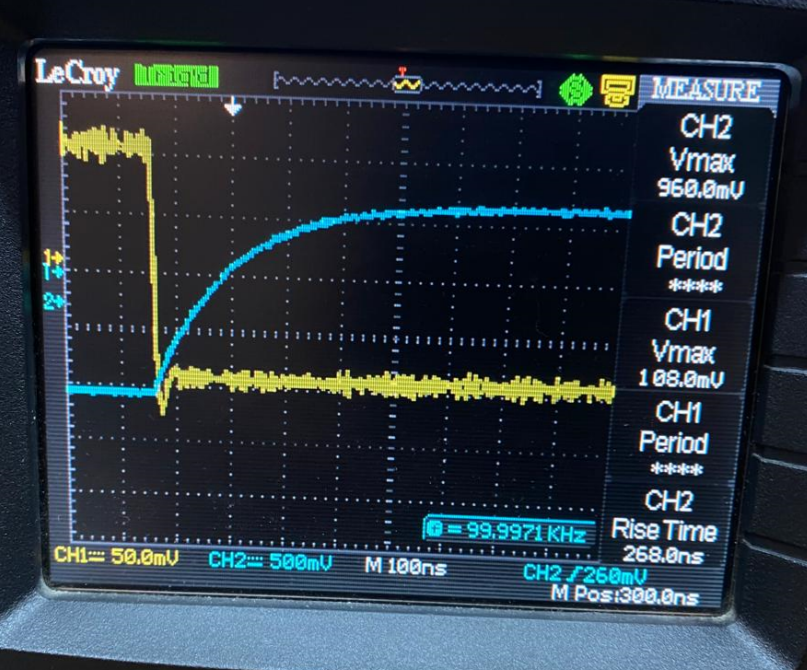
\includegraphics[width=0.47\textwidth]{imagenes/tiempo de respuesta CASCODE.png}
  \caption{Se observa el tiempo de respuesta en la esquina inferior derecha, como "Rise Time"}
  \label{fig:tr_EC}
\end{figure}

El tiempo de respuesta medido para el Cascode fue $t_r = 268ns$.

\section{Mediciones y Resultados}

A continuación se muestran dos tablas. La Tabla \ref{tab:resultados_exp} contiene los resultados obtenidos experimentalmente para las configuraciones EC y Cascode. La tabla \ref{tab:resultados_teoricos} contiene los resultados obtenidos analíticamente en la sección \textit{Marco Teórico}.

\begin{table}[h]
\begin{center}
\begin{tabular}{|c||c|c|}
\hline
 & Emisor Común & Cascode \\
\hline
$A_v$ (freq. medias)  & $-7,8$ & $-7,7$ \\
\hline
$f_H$ [$MHz$] & $1,49$ & $1,55$ \\
\hline
$t_r [$ns$]$ & $304$ & $268$ \\
\hline
\end{tabular}
\end{center}
\caption{Resultados experimentales}
\label{tab:resultados_exp}
\end{table}

Primeramente se observa que la Ganancia de Tensión se mantuvo practicamente constante para ambas configuraciones, mientras que se logró un aumento del ancho de banda de aproximadamente $60kHz$ (Mejora del 4\%).
A su vez, se logró una reducción del tiempo de respuesta de $36ns$ (Mejora del 11\%)

\begin{table}[h]
\begin{center}
\begin{tabular}{|c||c|c|}
\hline
 & Emisor Común & Cascode \\
\hline
$A_v$ (freq. medias)  & $-9,25$ & $-9,2$ \\
\hline
$f_H$ [$MHz$] & $1,444$ & $1,731$ \\
\hline
$t_r [$ns$]$ & $242$ & $202$ \\
\hline
\end{tabular}
\end{center}
\caption{Resultados teóricos esperados.}
\label{tab:resultados_teoricos}
\end{table}

Se esperaba, según lo calculado, un aumento del $19,8\%$ del ancho de banda, ademas de una reducción del $16,5\%$ del tiempo de respuesta.
Con respecto a la ganancia, se esperaba que se mantenga constante para ambas configuraciones.\\

Si se comparan los valores medidos con los teóricos, el error en la ganancia fue de aproximadamente $18,5\%$ tanto para el EC como para el Cascode, mientras que el error relativo para la frecuencia de corte fue muy pequeño para el caso del EC $(3,1\%)$ y un poco mayor para el Cascode $(11,6\%)$.
Para el tiempo de respuesta, el error medido para el EC fue del $25,6\%$, y del $32,6\%$ para el Cascode.

\section{Conclusiones}

En sí, los resultados fueron los esperados con lo que respecta al aumento del ancho de banda, la reducción del tiempo de respuesta, y la invariabilidad de la ganancia.\\
Ahora, teniendo en cuenta qué tan buena es dicha mejora, los experimentos realizados demuestran que el aumento de casi el $20\%$ del ancho de banda no sucedió, sino que fue mucho menor (alrededor del $4\%$), por lo que quizá para muchas aplicaciones, esta configuración quizá no sea la adecuada para aumentar el rango de frecuencias de operación.
Con respecto al tiempo de respuesta, el aumento fue del $11\%$, que es un aumento poco mas consideable.

\addtolength{\textheight}{-12cm}   % This command serves to balance the column lengths
                                  % on the last page of the document manually. It shortens
                                  % the textheight of the last page by a suitable amount.
                                  % This command does not take effect until the next page
                                  % so it should come on the page before the last. Make
                                  % sure that you do not shorten the textheight too much.

%%%%%%%%%%%%%%%%%%%%%%%%%%%%%%%%%%%%%%%%%%%%%%%%%%%%%%%%%%%%%%%%%%%%%%%%%%%%%%%%



%%%%%%%%%%%%%%%%%%%%%%%%%%%%%%%%%%%%%%%%%%%%%%%%%%%%%%%%%%%%%%%%%%%%%%%%%%%%%%%%



%%%%%%%%%%%%%%%%%%%%%%%%%%%%%%%%%%%%%%%%%%%%%%%%%%%%%%%%%%%%%%%%%%%%%%%%%%%%%%%%



%\section*{ACKNOWLEDGMENT}

%The preferred spelling of the word Òacknowledgment\'o in America is without an Òe\'o after the Òg\'o. Avoid the stilted expression, ÒOne of us (R. B. G.) thanks . . .\'o  Instead, try ÒR. B. G. thanks\'o. Put sponsor acknowledgments in the unnumbered footnote on the first page.



%%%%%%%%%%%%%%%%%%%%%%%%%%%%%%%%%%%%%%%%%%%%%%%%%%%%%%%%%%%%%%%%%%%%%%%%%%%%%%%%


\begin{thebibliography}{99}

\bibitem{c1} J. Millman and A. Grabel, ``Microelectrónica,” McGraw-Hill, New York, 6ta edición, 1993.
\bibitem{c2} P. R. Gray and R. G. Meyer, ``Analysis and Design of Analog Integrated Circuits,” John Wiley & Sons, New York, 4th edition, 2001



\end{thebibliography}




\end{document}
